\documentclass[useAMS,usenatbib]{mn2e}
\usepackage{myaasmacros}
\usepackage{graphicx}
\usepackage{ulem}
\usepackage{amsmath}


% Some definitions of things I always use here:
\def\ltsima{$\; \buildrel < \over \sim \;$}
\def\simlt{\lower.5ex\hbox{\ltsima}}   
\def\gtsima{$\; \buildrel > \over \sim \;$}
\def\simgt{\lower.5ex\hbox{\gtsima}}
\newcommand\bcite[1]{\citeauthor{#1} \citeyear{#1}}

% Some definitions for the priors:
\def\gprior{{\tt gprior}}
\def\cprior{{\tt cprior}}
\def\bprior{{\tt bprior}}
\def\lbprior{{\tt lbprior}}

%Some definitions for rhodm etc:
\def\vztwo{\overline{v_z^2}}
\def\vztwoi{\overline{v_{z,i}^2}}
\def\rhodisc{\rho_\mathrm{disc}(z)}
\def\rhodmext{\rho_\mathrm{dm,ext}}
\def\rhodm{\rho_\mathrm{dm}}
\def\rhoeff{\rho_\mathrm{dm}^\mathrm{eff}}
\def\nuobs{\nu_\mathrm{obs}(z)}

\title[Alignment of Light and Mass in Lensing Galaxies]{Alignment of Light and Mass in Lensing Galaxies}

\author[Bruderer]{Claudio Bruderer$^1$\thanks{E-mail: claudio.bruderer@phys.ethz.ch}, J. I. Read$^{1,2}$, P. Saha$^3$, J. Coles$^3$\\
$^1$Institute for Astronomy, Department of Physics, ETH Z\"urich, Wolfgang-Pauli-Strasse 27, CH-8093 Z\"urich, Switzerland\\
$^2$Department of Physics, University of Surrey, Guildford, GU2 7XH, UK\\
$^3$Institute for Theoretical Physics, University of Z\"urich, Winterthurerstrasse 190, 8057 Z\"urich, Switzerland
}

\begin{document}

\maketitle

\begin{abstract}
Abstract here. 
\end{abstract}

\begin{keywords}
\end{keywords}

\section{Introduction}

\subsection{Context/Background/Motivation}
\begin{itemize}
\item Why interesting (lensing can constrain mass distribution (enclosed mass constraint independent from model with only few percent uncertainty e.g. Kochanek 1991?, Wambsganss \& Paczyński 1994?), insights into structure formation)
\item What is to be expected from theory (dm, alternative gravity)
\end{itemize}


\subsection{Anything done before?}
\begin{itemize}
\item Surely cite: \cite{1997ApJ...482..604K,1998ApJ...509..561K,2006ApJ...649..599K,2009ApJ...690..670T,2012ApJ...761..170G}
\end{itemize}


\subsection{New here}
\begin{itemize}
\item Statistics
\item Free-form modelling
\item group versus stellar misalignment with dm halo
\end{itemize}



\section{Data}
\begin{itemize}
\item SPS (Ignacio Ferreras, Dominik, etc. \citep{2011ApJ...740...97L})
\item Write why specifically these lenses were chosen, where they're from
\end{itemize}



\begin{table}
 \begin{center}
  \begin{tabular}{l c c l | l c c l}
   Lens & $z_{L}$ & $z_{S}$ & Type & Lens & $z_{L}$ & $z_{S}$ & Type\\ \hline \hline
   Q0047 & 0.48 & 3.60 & Quad & HE1104 & 0.73 & 2.32 & Double\\
   Q0142 & 0.49 & 2.72 & Double & PG1115 & 0.31 & 1.72 & Quad\\
   MG0414 & 0.96 & 2.64 & Quad & B1152 & 0.44 & 1.02 & Double\\
   B0712 & 0.41 & 1.34 & Quad & B1422 & 0.34 & 3.62 & Quad\\
   RXJ0911 & 0.77 & 2.80 & Quad & B1608 & 0.63 & 1.39 & Quad\\
   BRI0952 & 0.63 & 4.50 & Double & MG2016 & 1.01 & 3.27 & Quad$^{1}$\\
   Q0957 & 0.36 & 1.41 & Double & B2045 & 0.87 & 1.28 & Quad\\
   LBQS1009 & 0.87 & 2.74 & Double & HE2149 & 0.60 & 2.03 & Double\\
   B1030 & 0.60 & 1.54 & Double & Q2237 & 0.04 & 1.69 & Quad\\
%   SBS1520 & 0.72 & 1.86 & Double
%	B1600 & 0.41 & 1.59 & Double\\
  \end{tabular}
  \caption{List of all the lenses in the sample and their properties. Data is taken from \textit{CASTLES} and \cite{leier11phd}. The angles are measured north-through-east. \newline $^{1}$ Two images merge, thus only three images can be resolved.}
  \label{tab:overview}
 \end{center}
\end{table}

\begin{table}
 \begin{center}
  \begin{tabular}{l c c c c c c c}
   \multirow{2}{*}{Lens} & \multirow{2}{*}{Environment$^{a}$} & \multicolumn{2}{c}{Group/Cluster centroid$^{b}$} & & \multicolumn{2}{c}{Other galaxy} & \multirow{2}{*}{References$^{c}$}\\ \cline{3-4} \cline{6-7}
    & & $\Delta\alpha$ [''] & $\Delta\delta$ [''] & & $\Delta\alpha$ [''] & $\Delta\delta$ ['']\\ \hline \hline
   Q0047 & G(9) & $3.6\pm15.6$ & $43.2\pm28.8$ &   & ... & ... & 1\\
   MG0414 & 2 & ... & ... &   & $-0.4$ & $1.5$ & 2\\
   B0712 & 2 & ... & ... &   & $47$ & $-91$ & 3\\
   RXJ0911 & C & $-12.0$ & $-39.8$ &    & ... & ... & 4\\
   Q0957 & C & ... & ... &   & ... & ... & 5\\
   B1030 & 2 & ... & ... &   & $-9.8$ & $8.5$ & 6\\
   PG1115 & G(13) & $-10.8\pm21.0$ & $-3.6\pm15.6$ &   & ... & ... & 1\\
   B1422 & G(17) & $61.2\pm25.2$ & $-10.8\pm23.4$ &   & ... & ... & 1\\
%   SBS1520 & G(5) & ... & ... &   & ... & ... & 7\\
%   B1600 & G(17) & $-8.4^{d}$ & $-1.5^{d}$ &   & ... & ... & 8\\
   B1608 & G(8) & $-0.7$ & $8.0$ &   & ... & ... & 9\\
   MG2016 & C(69) & ... & ... &   & ... & ... & 10\\
   HE2149 & G & $-36.6$ & $14.2$ &   & ... & ... & 11\\
  \end{tabular}
  \caption{List of lenses lying in a group or cluster environment, or that have a companion. \newline $^{a}$ G stands for group, C for cluster, and 2 means that the lens has a companion galaxy. If known, the number of member galaxies including the lens is given. \newline $^{b}$ If not stated differently, the centroid positions are luminosity-weighted estimates. \newline $^{c}$ References for the centroid estimates we used. \newline $^{d}$ Only number-weighted estimates are available. \newline 1: \cite{2011ApJ...726...84W}; 2: \cite{1993AJ....105....1S}; 3: \cite{2002AJ....123..627F}; 4: \cite{2001ApJ...555....1M}; 5: \cite{1998ApJ...504..661C}; 6: \cite{2000ApJ...536..584L}; 7: \cite{2008ApJ...673..778A}; 8: \cite{2007AJ....134..668A}; 9: \cite{2003MNRAS.344..337T}; 10: \cite{2006ApJ...646...85W}; 11: \cite{2006ApJ...646...85W}}
  \label{tab:environment}
 \end{center}
\end{table}

\begin{table}
 \begin{center}
  \begin{tabular}{l c c c c}
   Lens & \multicolumn{3}{c}{Time delays [d]} & References\\ \hline \hline
   RXJ0911 & $\Delta t_{BA}=146\pm4$ & ... & ... & 1\\
   Q0957 & $\Delta t_{BA}=416.5\pm1.0^{a}$ & $\Delta t_{BA}=420.6\pm1.9^{b}$ & ... & 2\\
   HE1104 & $\Delta t_{BA}=162.2^{+6.3}_{-5.9}$ & ...  & ...  & 3\\
   PG1115 & $\Delta t_{BA}=12.0^{+2.4}_{-2.0}$ & $\Delta t_{DC}=4.4^{+3.2}_{-2.4}$ & ... & 4\\
%   SBS1520 & $\Delta t_{BA}=125.8\pm2.1$ & ... & ... & 5\\
%   B1600 & $\Delta t_{BA}=51\pm2$ & ... & ... & 6\\
   B1608 & $\Delta t_{BA}=31.5^{+2}_{-1}$ & $\Delta t_{CA}=36.0\pm1.5$ & $\Delta t_{DA}=77.0^{+2}_{-1}$ & 7\\
   HE2149 & $\Delta t_{BA}=103\pm12$ & ... & ... & 8\\
  \end{tabular}
  \caption{Lenses with measured time delays. $\Delta t_{BA}$ corresponds to the time delay between the images A and B with A leading. \newline $^{a}$ measured in the g-band \newline $^{b}$ measured in the r-band \newline 1: \cite{2002ApJ...572L..11H}; 2: \cite{2012A&A...540A.132S}; 3: \cite{2008ApJ...676...80M}; 4: \cite{2010MNRAS.406.2764T}; 5: \cite{2011A&A...536A..44E}; 6: \cite{2000ApJ...544..117B}; 7: \cite{2002ApJ...581..823F}; 8: \cite{2002A&A...383...71B}}
  \label{tab:timedelays}
 \end{center}
\end{table}

The pixelated stellar mass maps we use, were reconstructed by \cite{leier11phd}. For each pixel the surface brightness was compared with stellar mass-to-light ratios, which were determined by stellar population synthesis models. This technique allows estimating the stellar mass in these pixels. Further details on this method can be found in \cite{leier11phd}, \cite{2005ApJ...623L...5F}, \cite{2008MNRAS.383..857F}.

Our sample consists of 20 galaxies. The sample is identical to the one as in \cite{leier11phd} and \cite{2011ApJ...740...97L} except that \textit{HS0818+1227} proved too difficult to reconstruct and therefore was left out. Most of the lens galaxies are early-type galaxies, except \textit{B1030+074}, \textit{B1152+200}, \textit{B1600+434}, \textit{B1608+656}, and \textit{Q2237+030}. All lenses can also be found in the gravitational lens database \textit{CASTLES}. Characteristics and references of each lens in the sample are listed below. Table \ref{tab:overview} contains of all the redshifts and the type of the lenses, Table \ref{tab:environment} lenses with environment information, and Table \ref{tab:timedelays} lenses with measured time delays.

\textit{Q0047-2808} (hereafter \textit{Q0047}) is a luminous early-type galaxy \citep{1996MNRAS.278..139W}. \cite{2011ApJ...726...84W} find a group of 9 members all of which they spectroscopically confirm.

\textit{Q0142-100} (hereafter \textit{Q0142}) is a passively evolving early-type galaxy according to \citep{2000ApJ...536..584L,2007A&A...465...51E}.

\textit{MG0414+0534} (hereafter \textit{MG0414}) is a passively evolving early-type galaxy \citep{1999AJ....117.2034T}. \cite{1993AJ....105....1S} find a very close luminous satellite galaxy north-west of the lens. Due to the proximity of this satellite, we include it as a point mass in our analysis.

\textit{B0712+472} (hereafter \textit{B0712}) is an early-type galaxy \citep{1998AJ....115..377F}. Another galaxy, 102'' to the south-east seems to be at a similar redshift \citep{2002AJ....123..627F}. There is also a group of 10 galaxies at a lower redshift.

\textit{RXJ0911+0551} (hereafter \textit{RXJ0911}) is an almost circular early-type galaxy \citep{2012A&A...538A..99S}. It has measured time delays \citep{2002ApJ...572L..11H}. It lies on the outskirts of a cluster \citep{2001ApJ...555....1M}. This cluster seems to be rather complex and especially it is not spherical. Possibly it is not dynamically relaxed, although X-ray emission can be detected. Analysis of this emission yields a temperature of 2.3 keV. There is also a satellite galaxy to the north-west direction \citep{2000ApJ...544L..35K}.

\textit{BRI0952-0115} (hereafter \textit{BRI0952}) is an early-type galaxy \citep{2000ApJ...536..584L,2007A&A...465...51E}. \cite{2006ApJ...641..169M} find that the lens lies in a poor group of 5 members. However, a redshift of $z=0.41$ was used. According to \cite{2007A&A...465...51E}, the redshift is more likely to be $z=0.632$. They also find a system of 2 or 3 other galaxies at a slightly higher redshift of which the lens could be part of. The required external shear could be explained easily by a cosmic contribution \citep{2000ApJ...536..584L}. Therefore, we treat this lens as an isolated object.

\textit{Q0957+561} (hereafter \textit{Q0957}) is a cD galaxy lying close to the center of a cluster with a high sprial galaxy-fraction (e.g. \cite{1992MNRAS.254P..27G,1994A&A...291..411A,1998ApJ...504..661C}). Due to the large image separation, large physical scales are probed. As listed in Table 3 of \cite{2000ApJ...542...74K}, the position angles to the center of the cluster of earlier lens reconstructions range between 51.8 deg and 67.8 deg measured north-through-east. These results are consistent with the center of the X-ray emission from the cluster \citep{1998ApJ...504..661C}. The lens has a measured time delay, e.g. \citep{2012A&A...540A.132S}. They however also find a three-day lag between the g- and r-bands, and the estimates do not agree at the 2$\sigma$-level. They argue that this effect can be accounted for by the presence of a substructure and chromatic dispersion. We find that the results do not change significantly for either estimate and choose therefore the g-band measurement.

\textit{LBQS1009-0252} (hereafter \textit{LBQS1009}) is probably an early-type galaxy \citep{2000ApJ...536..584L}. \cite{2004A&A...428..741F} find no significant galaxy overdensity near the lens.

\textit{B1030+074} (hereafter \textit{B1030}) appears to have some substructure \citep{1998MNRAS.300..649X}. \cite{2000ApJ...536..584L} conclude that there are two distinct galaxies. The main one is a red, early-type galaxy. The other component seems to be fitted well by an exponential disk galaxy. They also conclude that no firm statements about the environment can be made. Although there is another galaxy nearby, it is too blue to be an early-type galaxy and thus they cannot estimate its shear contribution.

\textit{HE1104-1805} (hereafter \textit{HE1104}) is probably an early-type galaxy \citep{2000ApJ...536..584L,2000A&A...360..853C}. It has measured time delays \citep{2008ApJ...676...80M}. \cite{2000ApJ...536..584L} also seem to find a group environment. \cite{2004A&A...428..741F} however conclude that the photometric redshift measurements of these galaxies indicate that they are at a higher redshift and rather associated with the source. Nonetheless, their lens models, parametric and free-form, all require strong external shear.

\textit{PG1115+080} (hereafter \textit{PG1115}) is an early-type galaxy \citep{2005ApJ...626...51Y}. It has measured time delays. We use recent estimates of the time delays by \cite{2010MNRAS.406.2764T} which differ significantly from traditional values by e.g. \cite{1997ApJ...489...21B}. \cite{2006ApJ...641..169M} and \cite{2011ApJ...726...84W} analyzed the environment of the lens thouroughly. It is part of a small group of 13 members. \cite{2004ApJ...610..686G} detect also X-ray emission from the corresponding group, which yields a temperature of 0.8 keV.

\textit{B1152+200} (hereafter \textit{B1152}) seems to have a color consistent with a late-type or an irregular galaxy \citep{2000A&A...357..115T}. Not much seems to be known about the environment of the lens.

\textit{B1422+231} (hereafter \textit{B1422}) is an early-type galaxy \citep{1996ApJ...462L..53I}. Although there are measured time delays by \cite{2001MNRAS.326.1403P}, they are probably not to be trusted too much as they deviate significantly from theoretical expectations in \cite{2003AJ....126...29R}. An accurate measurement of the time delays would require time delay measurements on the scale of hours. \cite{2006ApJ...641..169M} find a group environment with 16 spectroscopically confirmed member galaxies. Using newer data, \cite{2011ApJ...726...84W} find an additional member. \cite{2004ApJ...610..686G} also detect X-ray emission from the corresponding group at a temperature of 1.0 keV.

%\textit{SBS1520+530} (hereafter \textit{SBS1520}) is an early-type galaxy, possibly with a disc \citep{2008ApJ...673..778A}. It has measured time delays \citep{2011A&A...536A..44E}. There is some uncertainty about the redshift of the galaxy. \cite{2002A&A...391..481B} find that their spectroscopic redshift estimate is consistent with $z=0.71$, which was measured first by \cite{1997A&A...318L..67C}. Both however also find a system at $z=0.82$, which could be the main lens. \cite{2002A&A...391..481B} however conclude that it is not associated with the lens. \cite{2008ApJ...673..778A} argue that a system they find at $z=0.76$ is more likely to be the lens, and the foreground system at $z=0.71$ is just a local perturber. Data seems however not conclusive. \cite{2008ApJ...673..778A} find and spectroscopically confirm a total of 3 groups along the line of sight. A poor group of 5 members is at $z=0.716$, another one with 13 members is at $z=0.758$, and a third group with 10 members is at a higher redshift $z=0.818$.

%\textit{B1600+434} (hereafter \textit{B1600}) is a nearly edge-on viewed late-type galaxy \citep{1997A&A...317L..39J}. The lens lies in a group with at least seven members, which all seem to be late-type galaxies \citep{2007AJ....134..668A}.

\textit{B1608+656} (hereafter \textit{B1608}) consists of two merging galaxies. The main galaxy is an early-type galaxy which is disrupted by a smaller, probably late-type galaxy \citep{2003ApJ...584..100S}. The system has measured time delays \citep{2002ApJ...581..823F}. The environment and the mass distribution along the line of sight have been analyzed by \cite{2006ApJ...642...30F}. They find a group with 8 resp. 9 members if the merging galaxies are counted as 2. No significant X-ray emission was detected from the surrounding group \citep{2005ApJ...625..633D}. Along the line of sight seem to be four other groups.

\textit{MG2016+112} (hereafter \textit{MG2016}) is a giant elliptical galaxy \citep{1984Sci...223...46L,1986AJ.....91..991S}. It is the farthest lens we consider in this sample. It lies in a cluster which consists of 69 probable galaxies \citep{2003MNRAS.344..337T}. The clusters shows a high density of galaxies close to the lens in a south-east direction.

\textit{B2045+265} (hereafter \textit{B2045}) is probably an elliptical galaxy \citep{2007MNRAS.378..109M}. \cite{1999AJ....117..658F} initially classified the galaxy as a late-type Sa galaxy, the velocity dispersion however seems too high. As the source redshift is rather low, a large lens mass is needed. \cite{2007MNRAS.378..109M} therefore conclude that it is more likely an elliptical galaxy. To the west of the lens, \cite{1999AJ....117..658F} find that a group at a similar redshift as the lens. \cite{2007MNRAS.378..109M} also find evidence for a dwarf satellite galaxy.

\textit{HE2149-2745} (hereafter \textit{HE2149}) is an early-type galaxy \citep{2007A&A...465...51E}. It has a measured time delay \citep{2002A&A...383...71B}. There is some uncertainty in estimating the lens' redshift. Initial estimates by \cite{1996A&A...315L.405W,2000ApJ...543..131K} found a probable redshift range of $\sim0.2-0.5$. By cross-correlating the lens spectrum with a template spectrum of an elliptical galaxy, \cite{2002A&A...383...71B} find that the redshift probably lies in the range $0.49\leq z \leq 0.60$, with the most likely redshift $z=0.495\pm0.01$. \cite{2007A&A...465...51E} however find that the redshift is more likely to be $z=0.603\pm0.001$. This would probably make the lens part of a poor group found by \cite{2006ApJ...641..169M} and \cite{2006ApJ...646...85W}. They also find two other groups at lower redshifts.

\textit{Q2237+030} (hereafter \textit{Q2237} or \textit{2237}) is a barred spiral \citep{1988AJ.....95.1331Y}. With only a redshift of $z=0.04$, it is the closest lens of the sample. Due to the low redshift, the probed physical scales are quite small. No further inquiries into the environment were made.

Further information about the sample can be found in \cite{leier11phd}, \cite{2011ApJ...740...97L}, and \cite{2012A&A...538A..99S}.

NOTE: Cannot use B1608, but I still left it in the sample as Fei probably will use the lens.


\section{Methods}
\subsection{GLASS}
\begin{itemize}
\item Explain GLASS briefly and link to fake data tests
\end{itemize}

\subsection{Priors and assumptions}
\begin{itemize}
\item Explain what priors were chosen to model the lenses
\end{itemize}

Basically always pixrad 12, shear left free for quads, shear limited for doubles to 0.01, local gradient 50 degrees, smoothening prior 2, time delays if known. Exceptions are few. For some quads symmetry prior, for one double 0.01 was not possible therefore chose 0.1.


\subsection{Shape measure}
\begin{itemize}
\item Explain shape measure
\item Link to tests on fake data
\item Include one plot of fake data test -> Jonathan
\item Illustrate everything with example lens PG1115.
\end{itemize}


\section{Results}
\begin{itemize}
\item Show some examples (stellar and dm contour plots, image of lens, arrival time surface, included mass)
\item Show money plots
\item Comment on a few lenses special lenses
\item Environmental effect?
\end{itemize}

\begin{figure}
 \begin{center}
  \hspace{-7mm}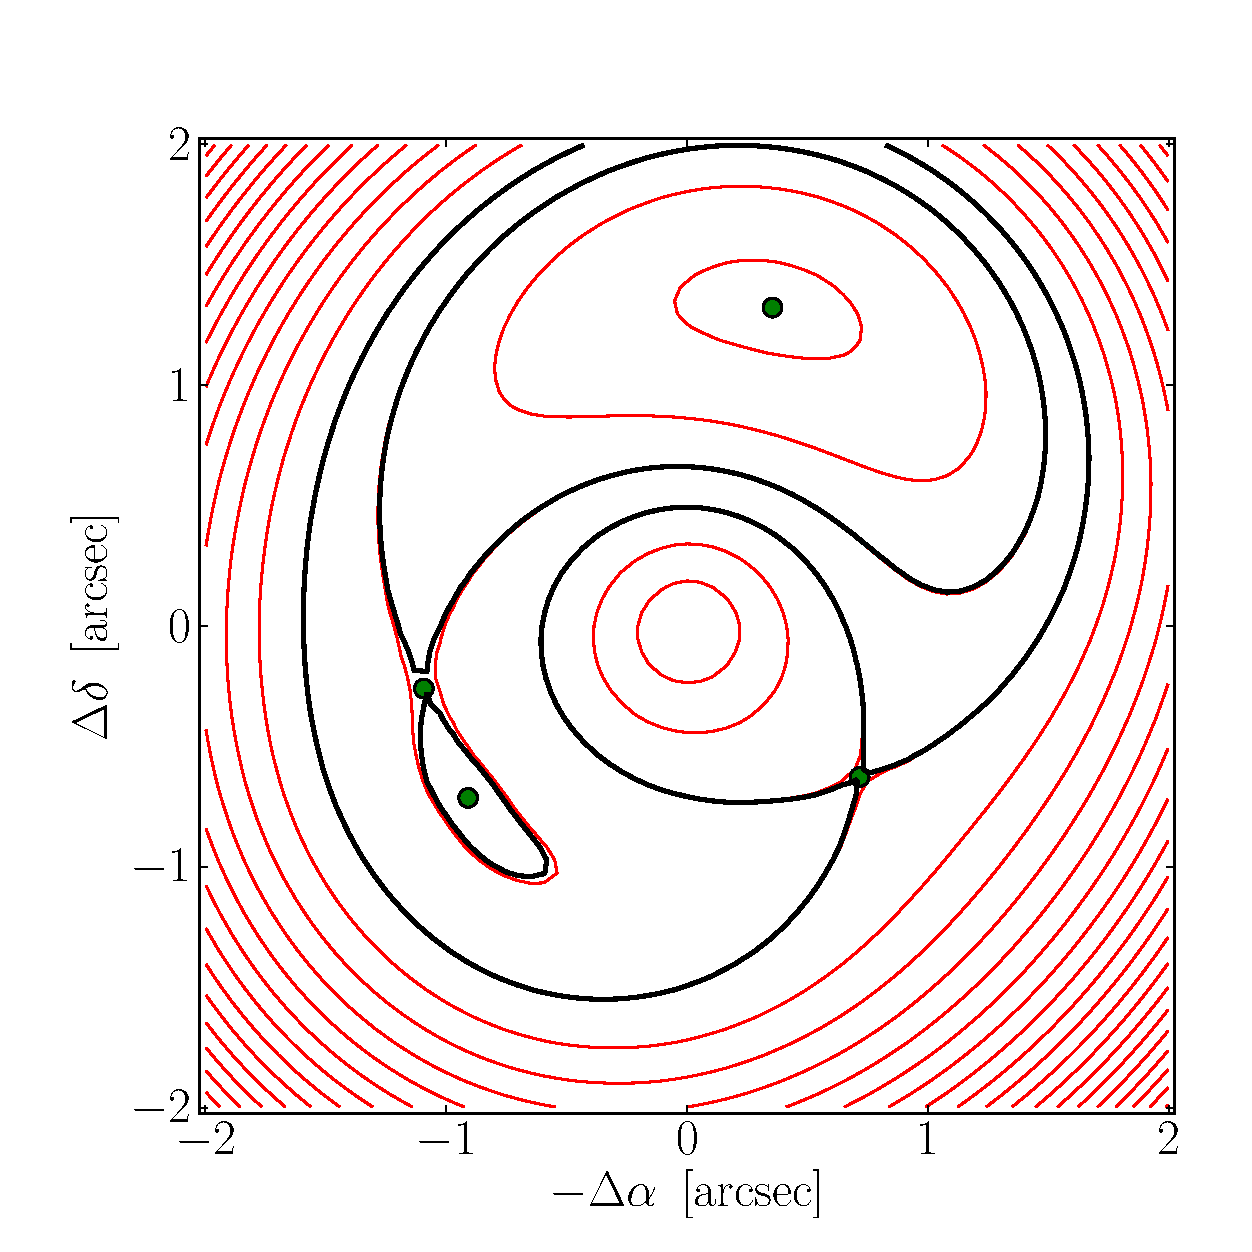
\includegraphics[height=0.1\textwidth]{Figures/1115_a.eps}
  \hspace{-7mm}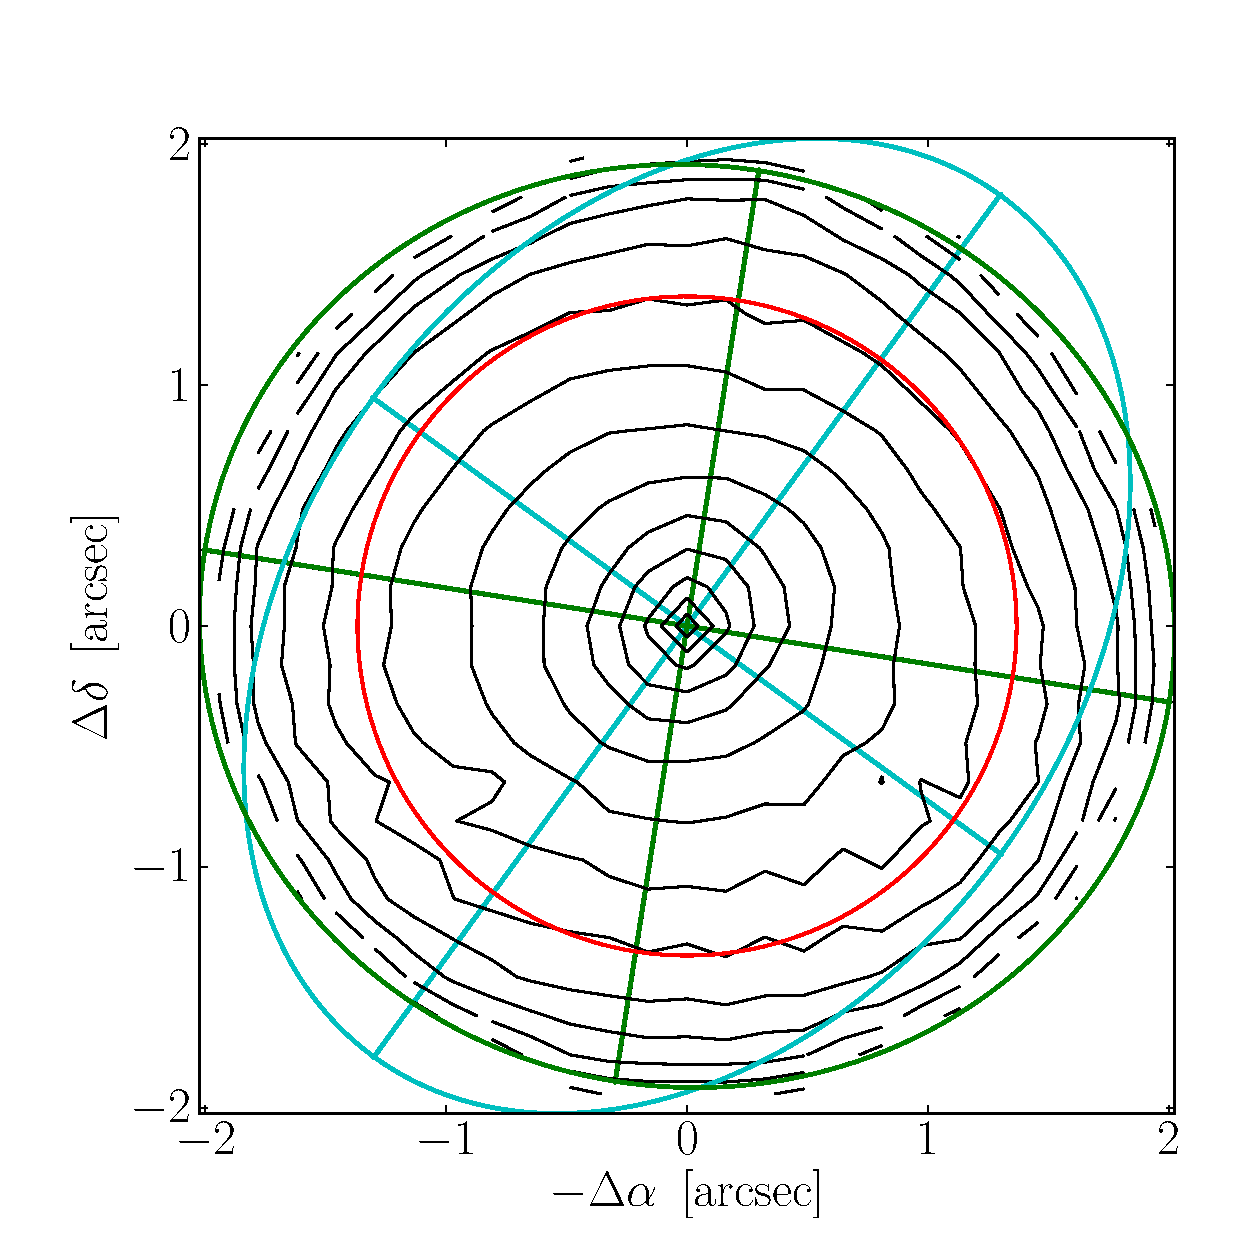
\includegraphics[height=0.1\textwidth]{Figures/1115_b.eps}
  \hspace{-7mm}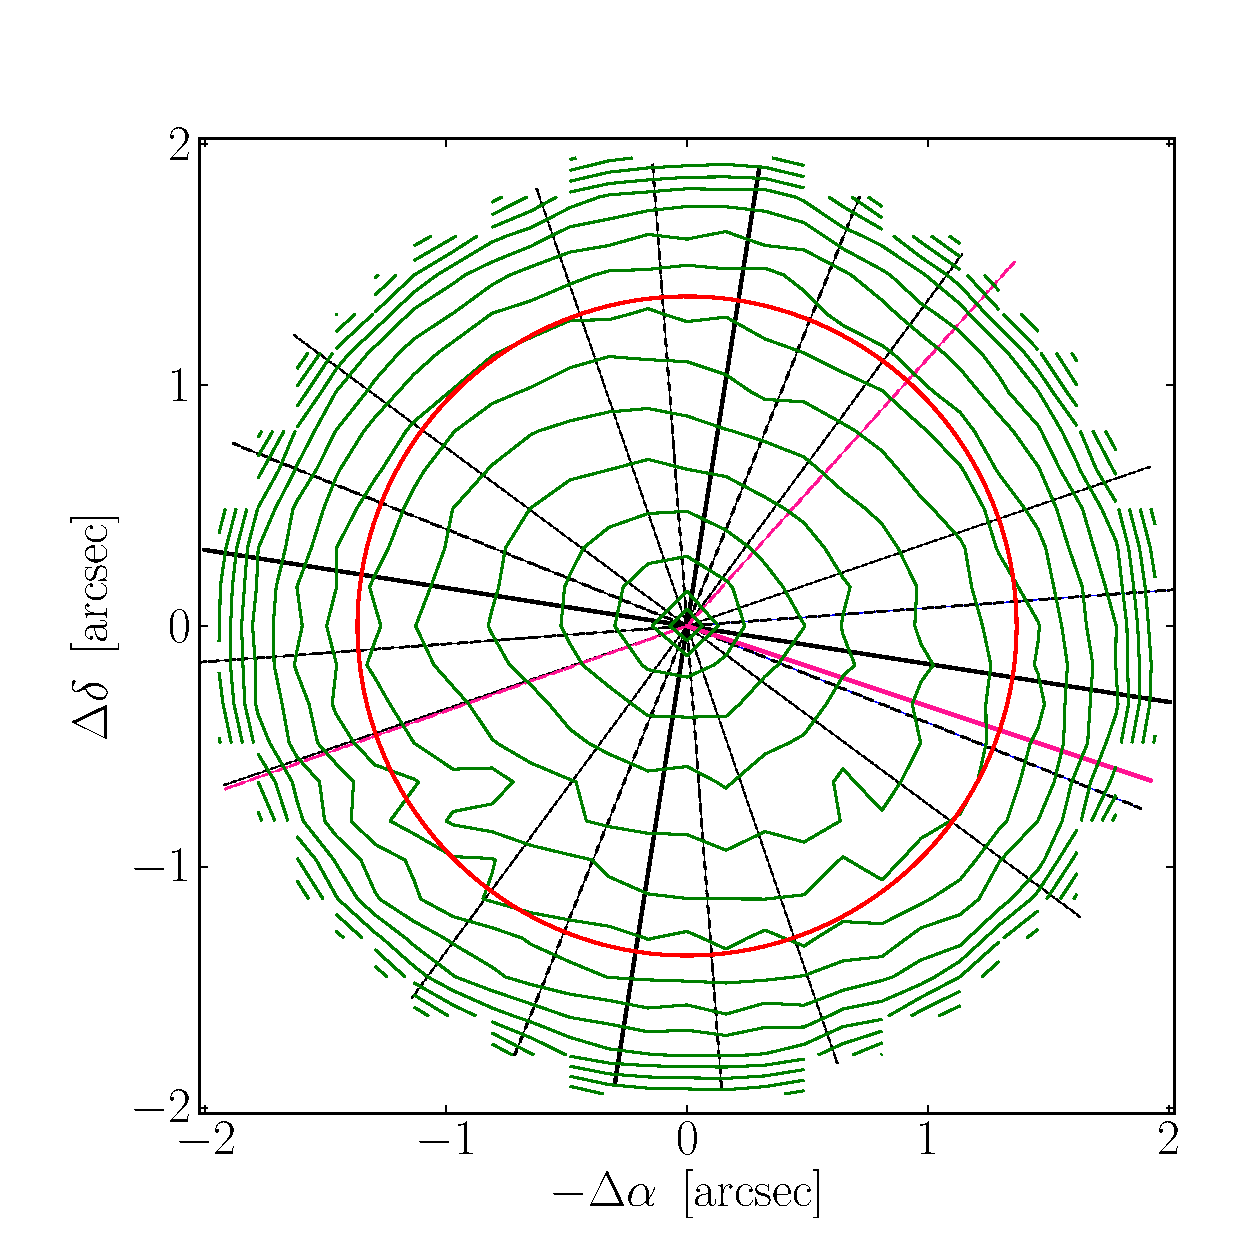
\includegraphics[height=0.1\textwidth]{Figures/1115_c.eps}
  \hspace{-7mm}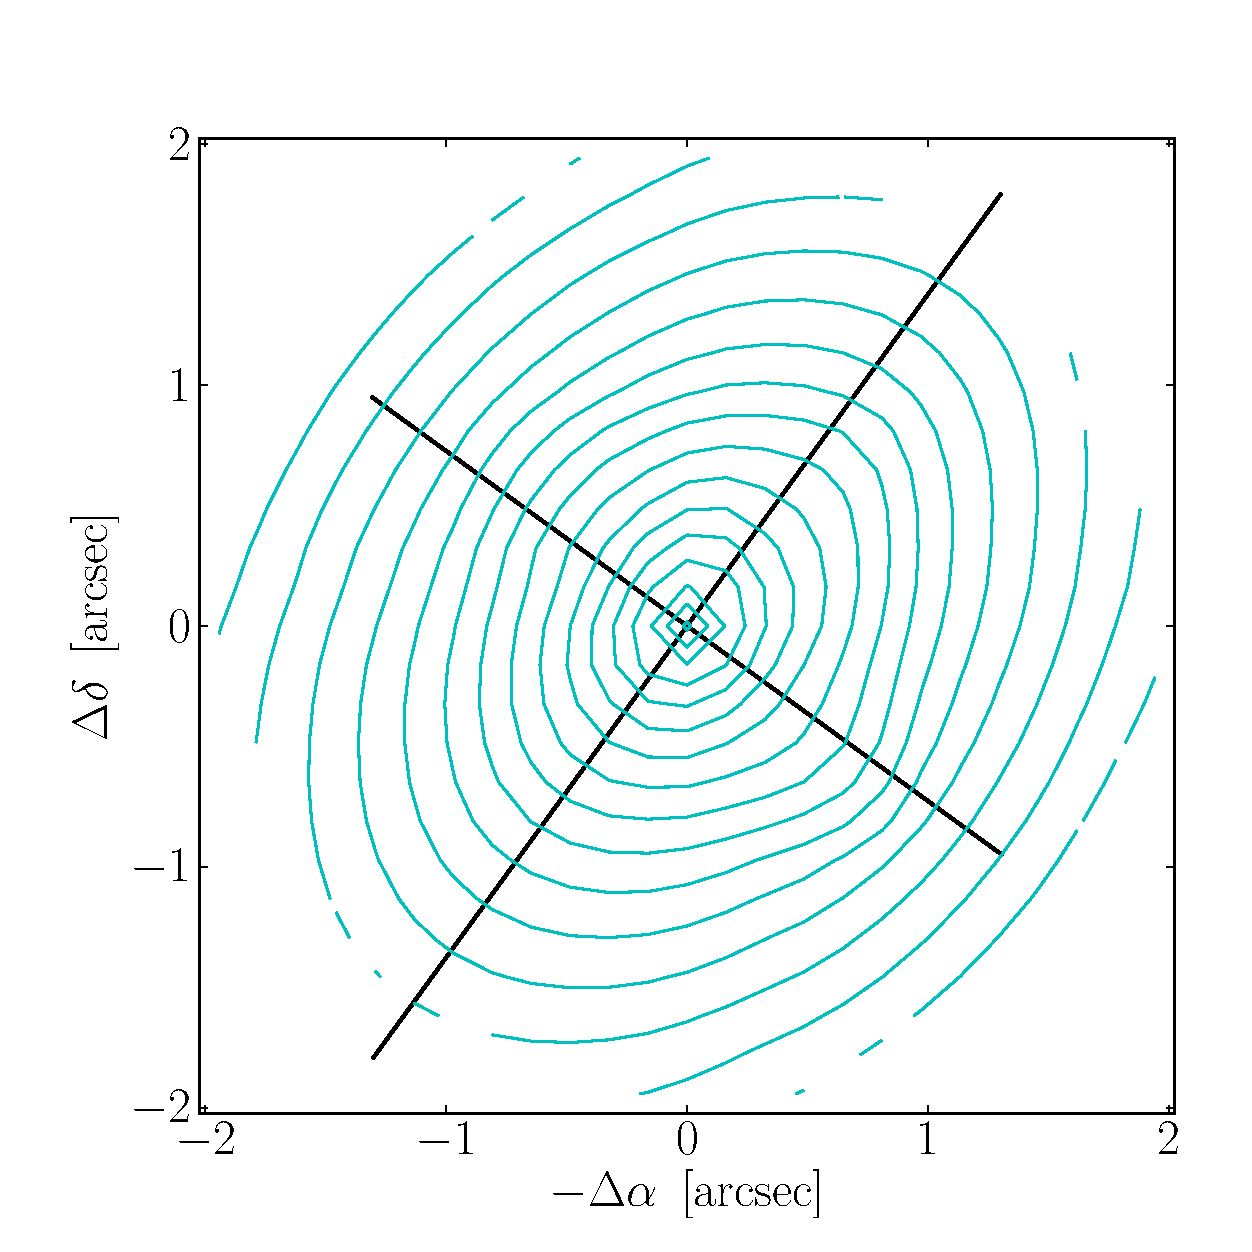
\includegraphics[height=0.1\textwidth]{Figures/1115_d.eps}
  \hspace{-7mm}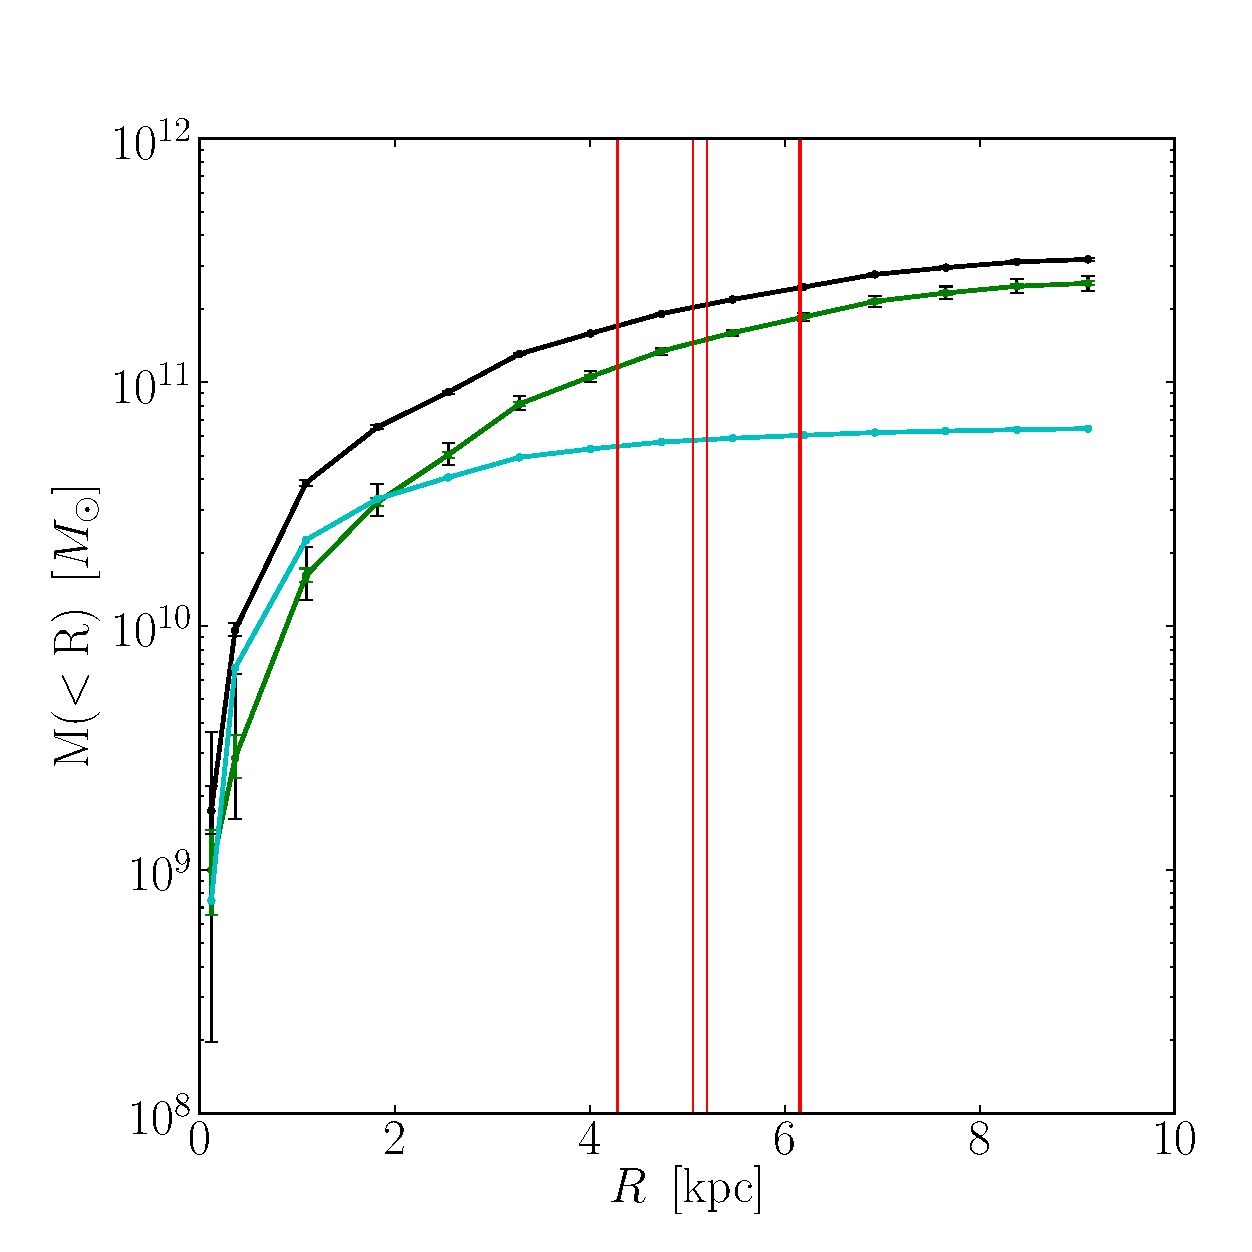
\includegraphics[height=0.1\textwidth]{Figures/1115_h.eps}\\
  \caption{Reconstruction of lens \textit{PG1115}}
  \label{fig:1115rec}
 \end{center}
\end{figure}

\begin{figure}
 \begin{center}
 \hspace{-7mm}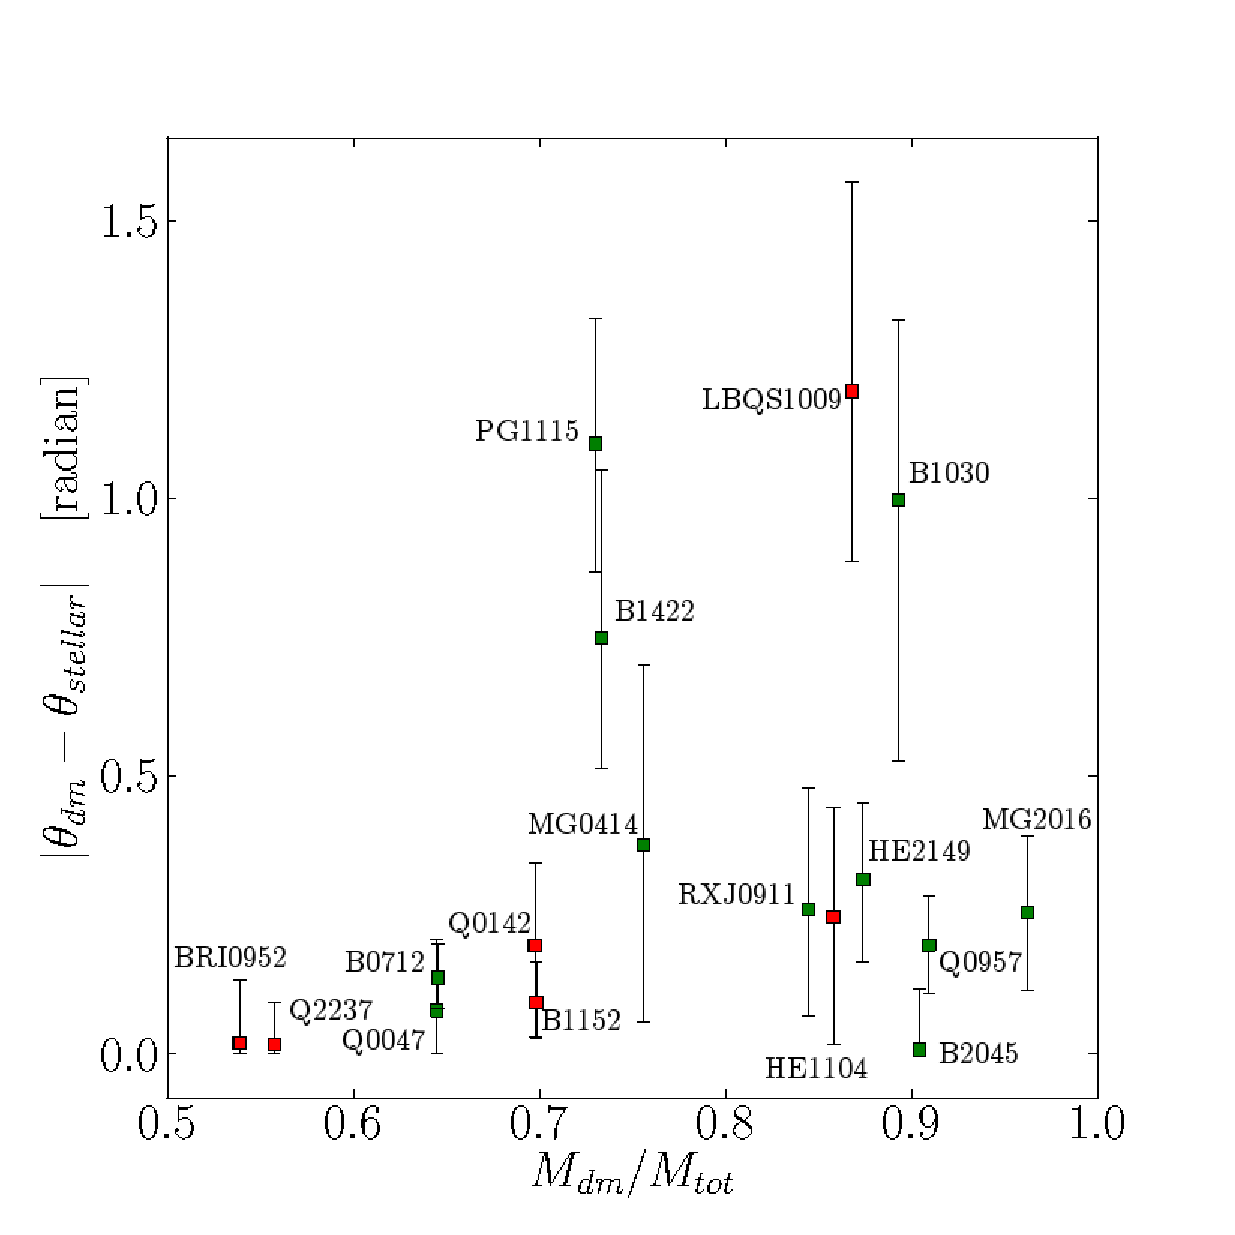
\includegraphics[height=0.29\textwidth]{Figures/b.eps}
 \hspace{-7mm}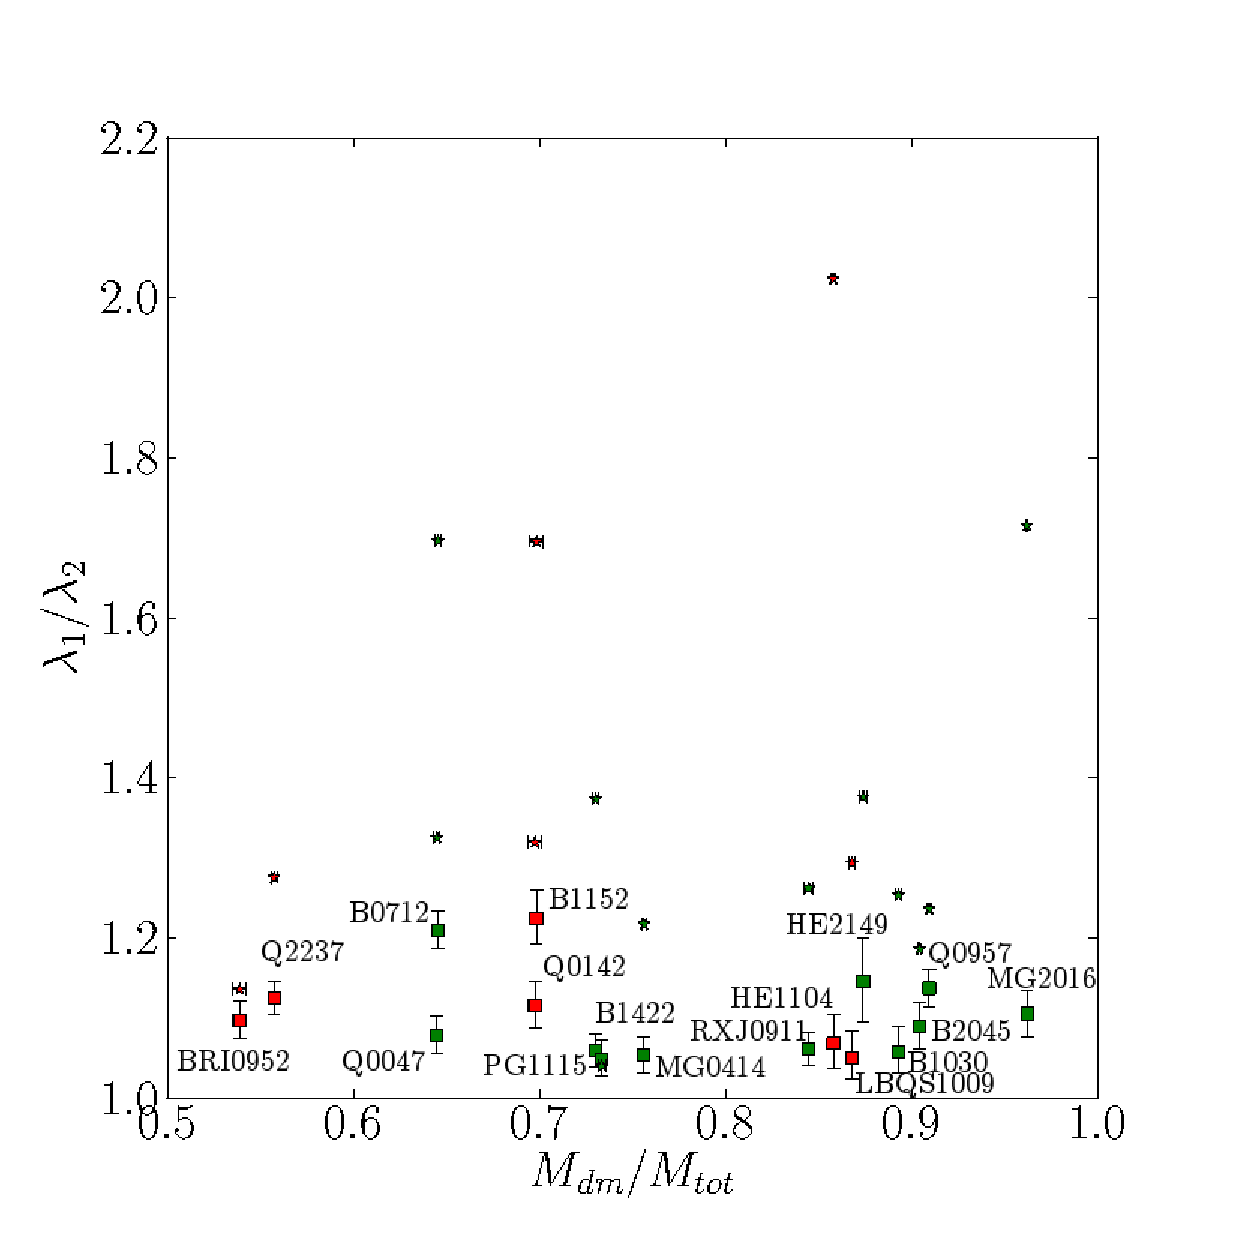
\includegraphics[height=0.29\textwidth]{Figures/d.eps}
 \hspace{-7mm}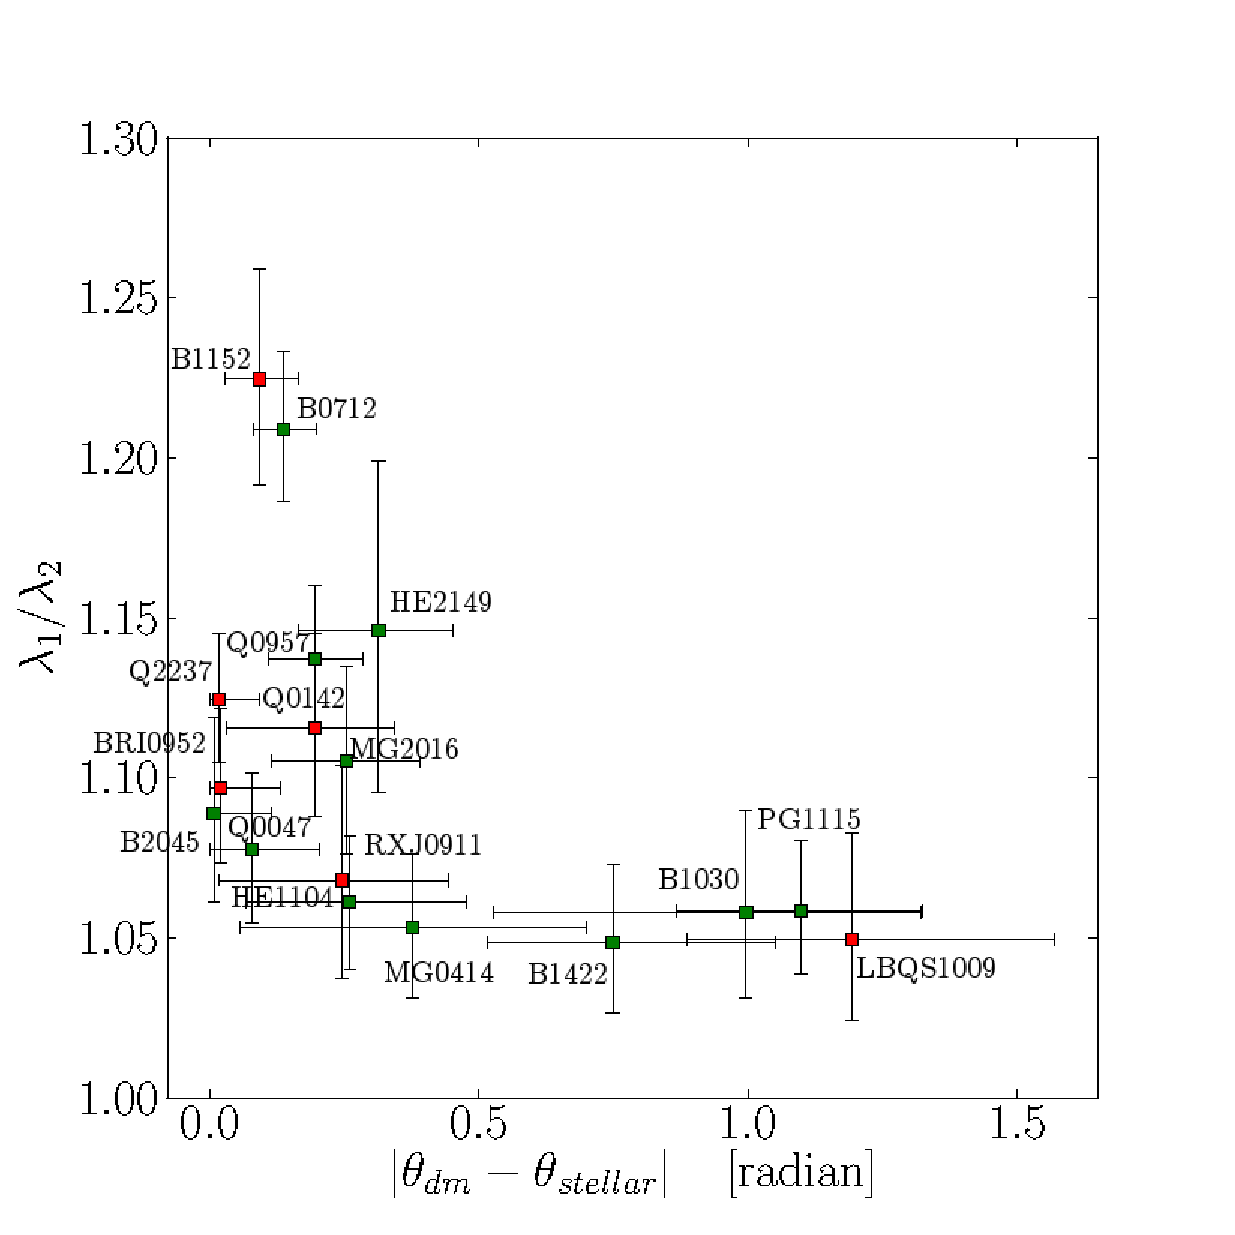
\includegraphics[height=0.29\textwidth]{Figures/e.eps}
 \caption{Plots of stellar and dark matter misalignments, ellipticities and composed plot.}
 \label{fig:moneyplots}
 \end{center}
\end{figure}

\begin{figure}
 \begin{center}
 \hspace{-7mm}\includegraphics[height=0.29\textwidth]{Figures/g.eps}
 \caption{Plots of stellar and dark matter misalignments, ellipticities and composed plot.}
 \label{fig:environmentmisalign}
 \end{center}
\end{figure}

\section{Conclusion}
\begin{itemize}
\item Recapitulate what were the main results
\item Answer whether this method is promising
\item What is needed to understand such misalignments better (-> Surely need to understand environment effects better, ...)
\end{itemize}

\section{Acknowledgements}
Acknowledge Dominik Leier...
JIR would like to acknowledge support from SNF grant PP00P2\_128540/1.

\bibliographystyle{mn2e}
\bibliography{paper.bib}

\end{document}
